\documentclass{standalone}
\usepackage{tikz}
\usetikzlibrary{patterns, positioning}


\begin{document}
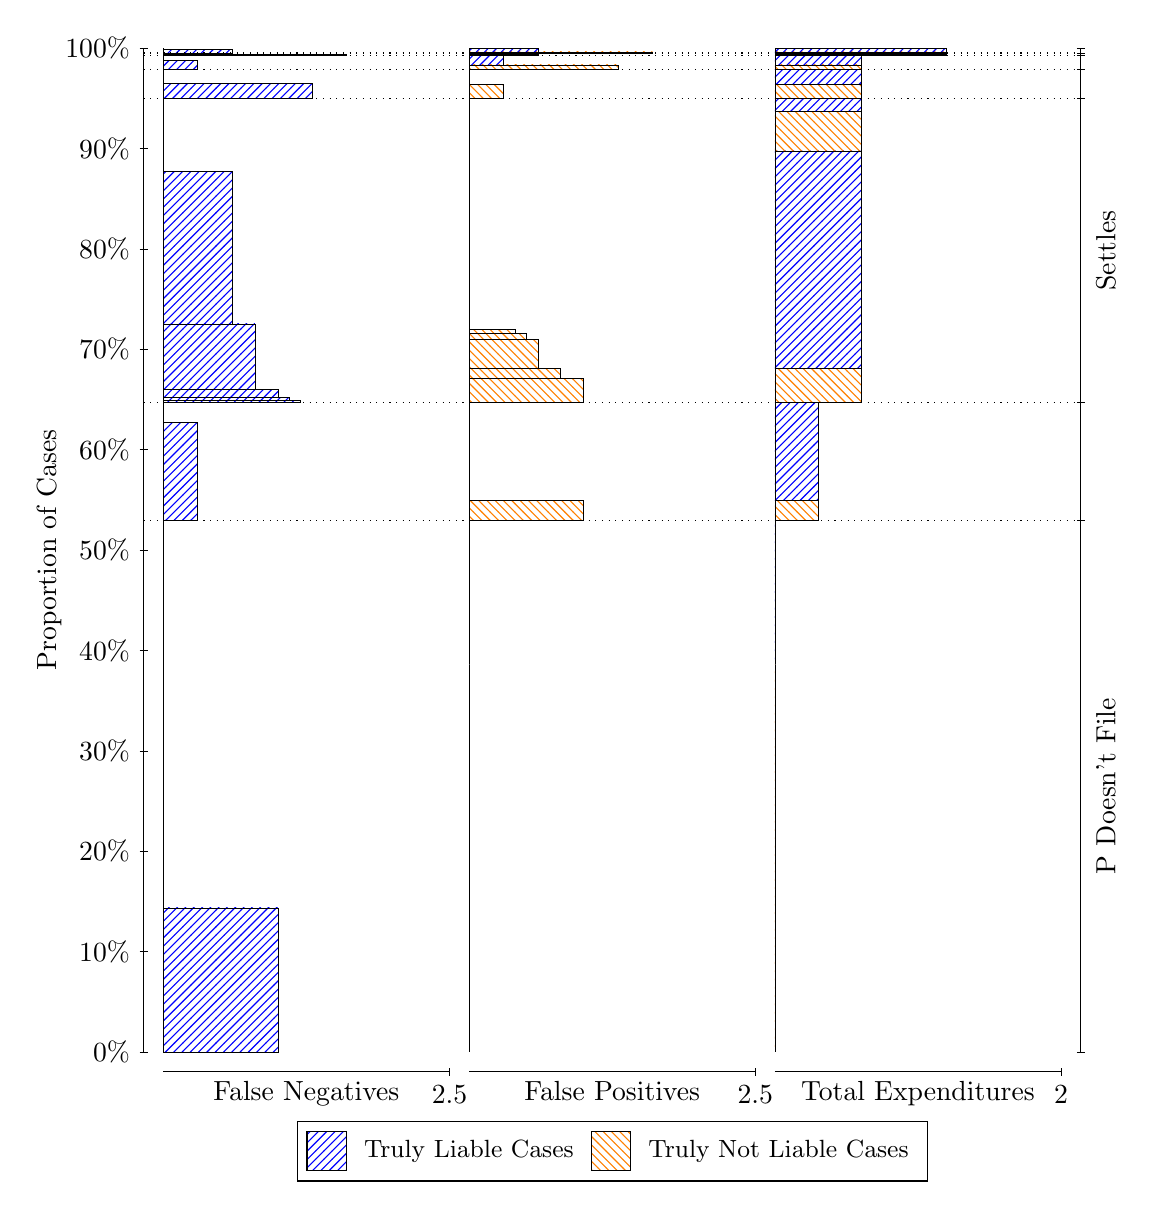
\begin{tikzpicture}
\draw[black, very thin] (1.5,1.75) -- (1.5,14.5);
\node[rotate=90, text=black, anchor=center] at (0.3, 8.125) {Proportion of Cases};
\draw[black, very thin] (1.45,1.75) -- (1.55,1.75);
\node[text=black, anchor=east] at (1.45, 1.75) {0\%};
\draw[black, very thin] (1.45,3.025) -- (1.55,3.025);
\node[text=black, anchor=east] at (1.45, 3.025) {10\%};
\draw[black, very thin] (1.45,4.3) -- (1.55,4.3);
\node[text=black, anchor=east] at (1.45, 4.3) {20\%};
\draw[black, very thin] (1.45,5.575) -- (1.55,5.575);
\node[text=black, anchor=east] at (1.45, 5.575) {30\%};
\draw[black, very thin] (1.45,6.85) -- (1.55,6.85);
\node[text=black, anchor=east] at (1.45, 6.85) {40\%};
\draw[black, very thin] (1.45,8.125) -- (1.55,8.125);
\node[text=black, anchor=east] at (1.45, 8.125) {50\%};
\draw[black, very thin] (1.45,9.4) -- (1.55,9.4);
\node[text=black, anchor=east] at (1.45, 9.4) {60\%};
\draw[black, very thin] (1.45,10.675) -- (1.55,10.675);
\node[text=black, anchor=east] at (1.45, 10.675) {70\%};
\draw[black, very thin] (1.45,11.95) -- (1.55,11.95);
\node[text=black, anchor=east] at (1.45, 11.95) {80\%};
\draw[black, very thin] (1.45,13.225) -- (1.55,13.225);
\node[text=black, anchor=east] at (1.45, 13.225) {90\%};
\draw[black, very thin] (1.45,14.5) -- (1.55,14.5);
\node[text=black, anchor=east] at (1.45, 14.5) {100\%};

\draw[black, very thin] (13.4,1.75) -- (13.4,14.5);
\draw[black, very thin] (13.35,1.75) -- (13.45,1.75);
\node[anchor=west] at (13.35, 1.75) {};
\draw[black, very thin] (13.35,8.502) -- (13.45,8.502);
\node[anchor=west] at (13.35, 8.502) {};
\draw[black, very thin] (13.35,10.001) -- (13.45,10.001);
\node[anchor=west] at (13.35, 10.001) {};
\draw[black, very thin] (13.35,13.858) -- (13.45,13.858);
\node[anchor=west] at (13.35, 13.858) {};
\draw[black, very thin] (13.35,14.229) -- (13.45,14.229);
\node[anchor=west] at (13.35, 14.229) {};
\draw[black, very thin] (13.35,14.402) -- (13.45,14.402);
\node[anchor=west] at (13.35, 14.402) {};
\draw[black, very thin] (13.35,14.437) -- (13.45,14.437);
\node[anchor=west] at (13.35, 14.437) {};
\draw[black, very thin] (13.35,14.5) -- (13.45,14.5);
\node[anchor=west] at (13.35, 14.5) {};

\draw[black, very thin, pattern color=blue, pattern=north east lines] (1.75,1.75) rectangle (3.2033,3.5792);
\draw[black, very thin, pattern color=orange, pattern=north west lines] (1.75,3.5792) rectangle (1.75,8.502);
\draw[black, very thin, pattern color=blue, pattern=north east lines] (1.75,8.502) rectangle (2.186,9.7462);
\draw[black, very thin, pattern color=orange, pattern=north west lines] (1.75,9.7462) rectangle (1.75,10.001);
\draw[black, very thin, pattern color=blue, pattern=north east lines] (1.75,10.001) rectangle (3.494,10.026);
\draw[black, very thin, pattern color=blue, pattern=north east lines] (1.75,10.026) rectangle (3.3487,10.065);
\draw[black, very thin, pattern color=blue, pattern=north east lines] (1.75,10.065) rectangle (3.2033,10.168);
\draw[black, very thin, pattern color=blue, pattern=north east lines] (1.75,10.168) rectangle (2.9127,10.997);
\draw[black, very thin, pattern color=blue, pattern=north east lines] (1.75,10.997) rectangle (2.622,12.932);
\draw[black, very thin, pattern color=orange, pattern=north west lines] (1.75,12.932) rectangle (1.75,13.858);
\draw[black, very thin, pattern color=blue, pattern=north east lines] (1.75,13.858) rectangle (3.6393,14.049);
\draw[black, very thin, pattern color=orange, pattern=north west lines] (1.75,14.049) rectangle (1.75,14.229);
\draw[black, very thin, pattern color=blue, pattern=north east lines] (1.75,14.229) rectangle (2.186,14.346);
\draw[black, very thin, pattern color=orange, pattern=north west lines] (1.75,14.346) rectangle (1.75,14.402);
\draw[black, very thin, pattern color=blue, pattern=north east lines] (1.75,14.402) rectangle (4.0753,14.417);
\draw[black, very thin, pattern color=orange, pattern=north west lines] (1.75,14.417) rectangle (1.75,14.437);
\draw[black, very thin, pattern color=blue, pattern=north east lines] (1.75,14.437) rectangle (2.622,14.485);
\draw[black, very thin, pattern color=orange, pattern=north west lines] (1.75,14.485) rectangle (1.75,14.5);
\draw[black, very thin, pattern color=orange, pattern=north west lines] (5.6333,1.75) rectangle (5.6333,6.6728);
\draw[black, very thin, pattern color=blue, pattern=north east lines] (5.6333,6.6728) rectangle (5.6333,8.502);
\draw[black, very thin, pattern color=orange, pattern=north west lines] (5.6333,8.502) rectangle (7.0867,8.757);
\draw[black, very thin, pattern color=blue, pattern=north east lines] (5.6333,8.757) rectangle (5.6333,10.001);
\draw[black, very thin, pattern color=orange, pattern=north west lines] (5.6333,10.001) rectangle (7.0867,10.302);
\draw[black, very thin, pattern color=orange, pattern=north west lines] (5.6333,10.302) rectangle (6.796,10.431);
\draw[black, very thin, pattern color=orange, pattern=north west lines] (5.6333,10.431) rectangle (6.5053,10.8);
\draw[black, very thin, pattern color=orange, pattern=north west lines] (5.6333,10.8) rectangle (6.36,10.872);
\draw[black, very thin, pattern color=orange, pattern=north west lines] (5.6333,10.872) rectangle (6.2147,10.927);
\draw[black, very thin, pattern color=blue, pattern=north east lines] (5.6333,10.927) rectangle (5.6333,13.858);
\draw[black, very thin, pattern color=orange, pattern=north west lines] (5.6333,13.858) rectangle (6.0693,14.038);
\draw[black, very thin, pattern color=blue, pattern=north east lines] (5.6333,14.038) rectangle (5.6333,14.229);
\draw[black, very thin, pattern color=orange, pattern=north west lines] (5.6333,14.229) rectangle (7.5227,14.285);
\draw[black, very thin, pattern color=blue, pattern=north east lines] (5.6333,14.285) rectangle (6.0693,14.402);
\draw[black, very thin, pattern color=orange, pattern=north west lines] (5.6333,14.402) rectangle (6.5053,14.422);
\draw[black, very thin, pattern color=blue, pattern=north east lines] (5.6333,14.422) rectangle (5.6333,14.437);
\draw[black, very thin, pattern color=orange, pattern=north west lines] (5.6333,14.437) rectangle (7.9587,14.452);
\draw[black, very thin, pattern color=blue, pattern=north east lines] (5.6333,14.452) rectangle (6.5053,14.5);
\draw[black, very thin, pattern color=orange, pattern=north west lines] (9.5167,1.75) rectangle (9.5167,6.6728);
\draw[black, very thin, pattern color=blue, pattern=north east lines] (9.5167,6.6728) rectangle (9.5167,8.502);
\draw[black, very thin, pattern color=orange, pattern=north west lines] (9.5167,8.502) rectangle (10.062,8.757);
\draw[black, very thin, pattern color=blue, pattern=north east lines] (9.5167,8.757) rectangle (10.062,10.001);
\draw[black, very thin, pattern color=orange, pattern=north west lines] (9.5167,10.001) rectangle (10.607,10.431);
\draw[black, very thin, pattern color=blue, pattern=north east lines] (9.5167,10.431) rectangle (10.607,13.195);
\draw[black, very thin, pattern color=orange, pattern=north west lines] (9.5167,13.195) rectangle (10.607,13.692);
\draw[black, very thin, pattern color=blue, pattern=north east lines] (9.5167,13.692) rectangle (10.607,13.858);
\draw[black, very thin, pattern color=orange, pattern=north west lines] (9.5167,13.858) rectangle (10.607,14.038);
\draw[black, very thin, pattern color=blue, pattern=north east lines] (9.5167,14.038) rectangle (10.607,14.229);
\draw[black, very thin, pattern color=orange, pattern=north west lines] (9.5167,14.229) rectangle (10.607,14.285);
\draw[black, very thin, pattern color=blue, pattern=north east lines] (9.5167,14.285) rectangle (10.607,14.402);
\draw[black, very thin, pattern color=orange, pattern=north west lines] (9.5167,14.402) rectangle (11.697,14.422);
\draw[black, very thin, pattern color=blue, pattern=north east lines] (9.5167,14.422) rectangle (11.697,14.437);
\draw[black, very thin, pattern color=orange, pattern=north west lines] (9.5167,14.437) rectangle (11.697,14.452);
\draw[black, very thin, pattern color=blue, pattern=north east lines] (9.5167,14.452) rectangle (11.697,14.5);
\draw[black, dotted] (1.5,8.502) -- (13.4,8.502);
\draw[black, dotted] (1.5,10.001) -- (13.4,10.001);
\draw[black, dotted] (1.5,13.858) -- (13.4,13.858);
\draw[black, dotted] (1.5,14.229) -- (13.4,14.229);
\draw[black, dotted] (1.5,14.402) -- (13.4,14.402);
\draw[black, dotted] (1.5,14.437) -- (13.4,14.437);
\draw[black, very thin] (1.75,1.5) -- (5.3833,1.5);
\node[text=black, anchor=north] at (3.5667, 1.5) {False Negatives};
\draw[black, very thin] (5.3833,1.45) -- (5.3833,1.55);
\node[text=black, anchor=north] at (5.3833, 1.45) {2.5};

\draw[black, very thin] (5.6333,1.5) -- (9.2667,1.5);
\node[text=black, anchor=north] at (7.45, 1.5) {False Positives};
\draw[black, very thin] (9.2667,1.45) -- (9.2667,1.55);
\node[text=black, anchor=north] at (9.2667, 1.45) {2.5};

\draw[black, very thin] (9.5167,1.5) -- (13.15,1.5);
\node[text=black, anchor=north] at (11.333, 1.5) {Total Expenditures};
\draw[black, very thin] (13.15,1.45) -- (13.15,1.55);
\node[text=black, anchor=north] at (13.15, 1.45) {2};

\node[text=black, centered, rotate=90] at (13.72, 5.126) {P Doesn't File};

\node[text=black, centered, rotate=90] at (13.72, 11.93) {Settles};





\draw (7.449999999999999,1.5) node[draw=none] (baseCoordinate) {};
\begin{scope}[align=center]
        \matrix[scale=0.5, draw=black, below=0.5cm of baseCoordinate, nodes={draw}, column sep=0.1cm]{
            \node[rectangle, draw, minimum width=0.5cm, minimum height=0.5cm, pattern color=blue, pattern=north east lines] {}; &
            \node[draw=none, font=\small, text=black] (B) {Truly Liable Cases}; &
            \node[rectangle, draw, minimum width=0.5cm, minimum height=0.5cm, pattern color=orange, pattern=north west lines] {}; &
            \node[draw=none, font=\small, text=black] (B) {Truly Not Liable Cases}; \\
            };
\end{scope}

\end{tikzpicture}
\end{document}